%%%%%%%%%%%%%%%%%%%%%%%%%%%%%%%%%%%%%%%%%%%%%%%%%%%%%%%%%%%%%%%%%%%%%%%%%%%%%%%
%%%%%%%%%%%%%%%%%%%%%%%%%%%%%%%%%%%%%%%%%%%%%%%%%%%%%%%%%%%%%%%%%%%%%%%%%%%%%%%
\documentclass[a4paper]{article}

\usepackage{graphicx}
\usepackage[utf8]{inputenc}
\usepackage[spanish]{babel}
\usepackage{pslatex}

\topmargin -10mm
\oddsidemargin 0.1in
\textwidth 6.0in
\textheight 9.5in
\parindent 0mm
\parskip 2mm
\pagestyle{empty}

\newcommand{\simbolo}[1]{\makebox[5mm][l]{
\setlength{\unitlength}{1mm}
\begin{picture}(0,0)
\put(0,1){\oval(4,4)}
\put(0,1){\makebox(0,0){#1}}
\end{picture}}}

\begin{document}

\centerline{\Large Programa {\sc ucmima}}

{\sc ucmima} es un programa sencillo para el an\'{a}lisis y manipulaci\'{o}n de
im\'{a}genes {\sc fits}, que funciona bajo sistema operativo {\sc unix}. El
profesor encargado de las pr\'{a}cticas de laboratorio asignar\'{a} a cada
grupo un directorio de trabajo, en el cual se introducir\'{a}n las
im\'{a}genes necesarias y se realizar\'{a} todo el trabajo.

El programa se ejecuta escribiendo su nombre (en min\'{u}sculas) en la
l\'{\i}nea de comandos, es decir:

{\tt \$ ucmima}

Instantes despu\'{e}s dispondremos de una ventana gr\'{a}fica con el aspecto
mostrado en la figura inferior. Conviene dedicar unos minutos a examinar las
diferentes posibilidades que el programa nos ofrece. Con ayuda del rat\'{o}n
podemos seleccionar la opci\'{o}n deseada, las cuales se muestran como botones
resaltados. Cada vez que una opci\'{o}n ha sido seleccionada, el bot\'{o}n
correspondiente permanece ``apretado'' hasta que la acci\'{o}n termina de
ejecutarse. Los botones se han agrupado en varios men\'{u}s:
\begin{itemize}
  \item {\sc archivo}: botones \simbolo{1}, \simbolo{2} y \simbolo{3}
  \item {\sc zoom}: botones \simbolo{4} y \simbolo{5}
  \item {\sc medir}: botones \simbolo{6} y \simbolo{7}
  \item {\sc calculadora}: botones \simbolo{8}, \simbolo{9} y \simbolo{10}
  \item cortes de la imagen: botones \simbolo{11}, \simbolo{12}, \simbolo{13} 
y \simbolo{14}
\end{itemize}
Una explicaci\'{o}n de la utilidad de todos los botones se indica en la figura.

\vspace{35mm}

\centerline{%
\resizebox{0.83\hsize}{!}{%
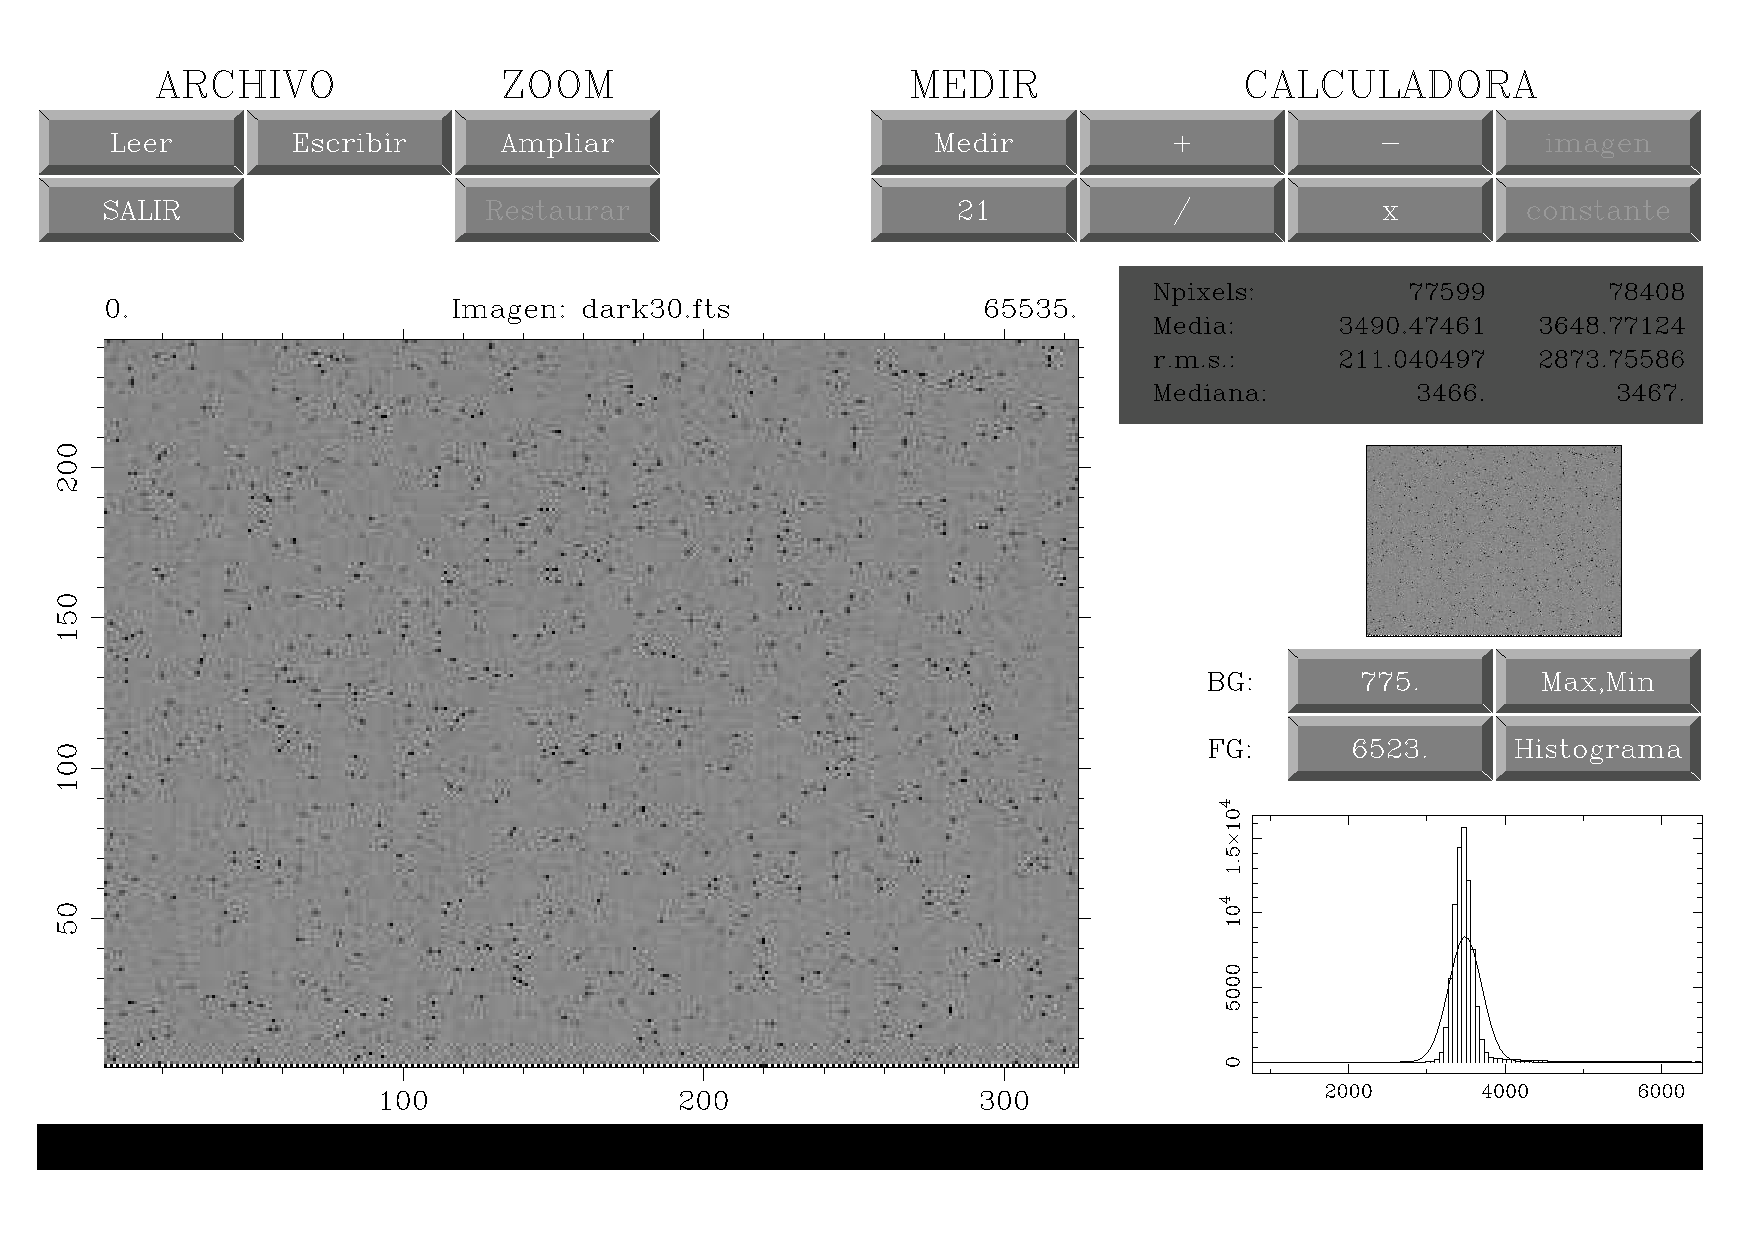
\includegraphics[angle=0]{sample.pdf}}%
}%end of centerline

\vspace{-105mm}

\setlength{\unitlength}{1mm}
\begin{picture}(160,100)
% escala cada 10 mm en cada eje
%\multiput(0,0)(10,0){17}{\line(0,1){100}}
%\multiput(0,0)(0,10){11}{\line(1,0){160}}

%------------------------------------------------------------------------------
% ARCHIVO
% Leer
\put(15,77){\vector(-1,1){5}}
\put(-16,82){\parbox{25mm}{\footnotesize \simbolo{1} lee una imagen en formato 
{\sc fits}}}
% Salir
\put(15,72){\vector(-1,-1){5}}
\put(-16,67){\parbox{25mm}{\footnotesize \simbolo{2} termina la ejecuci\'{o}n 
del programa}}
%Escribir
\put(40,80){\vector(-1,4){2.0}}
\put(18,87){\parbox[b]{25mm}{\footnotesize \simbolo{3} escribe la imagen actual
en un fichero en formato {\sc fits}}}

%------------------------------------------------------------------------------
% ZOOM
% Ampliar
\put(48,80){\vector(0,1){24}}
\put(35,102){\parbox[b]{25mm}{\footnotesize \simbolo{4} amplia una regi\'{o}n 
de la imagen con la ayuda del rat\'{o}n}}
\put(61,73){\line(1,0){5}}
\put(66,73){\vector(0,1){13}}
\put(53,87){\parbox[b]{25mm}{\footnotesize \simbolo{5} dibuja la ima\-gen 
com\-ple\-ta des\-pu\'{e}s de un zoom}}

%------------------------------------------------------------------------------
% MEDIR
% (21)
\put(76,73){\line(-1,0){5}}
\put(71,73){\line(0,1){7}}
\put(71,80){\line(2,1){10}}
\put(81,85){\vector(0,1){15}}
\put(68,102){\parbox[b]{30mm}{\footnotesize \simbolo{6} muestra el tama\~{n}o 
del cuadrado en el cual se mide y permite cambiar dicho valor}}
% Medir
\put(90,80){\vector(1,2){5}}
\put(85,91){\parbox[b]{28mm}{\footnotesize \simbolo{7} mide en un cuadrado de 
tama\~{n}o fijado por el bot\'{o}n \simbolo{6}}}

%------------------------------------------------------------------------------
% CALCULADORA
% (operaciones)
\put(98,80){\line(0,1){5}}
\put(98,85){\line(1,0){19}}
\put(117,80){\vector(0,1){23}}
\put(104,102){\parbox[b]{33mm}{\footnotesize \simbolo{8} operaciones 
ele\-men\-ta\-les (+,$-$,$\times$,$\div$) que pue\-den aplicarse a la imagen 
actual}}
% imagen
\put(135,80){\vector(0,1){5}}
\put(122,87){\parbox[b]{30mm}{\footnotesize \simbolo{9} la ope\-ra\-ci\'{o}n 
arit\-m\'{e}\-ti\-ca seleccionada se realiza usando una segunda imagen 
{\sc fits}}}
\put(137,73){\vector(1,0){4}}
\put(142,73){\parbox{27mm}{\footnotesize \simbolo{10} la ope\-ra\-ci\'{o}n 
arit\-m\'{e}\-ti\-ca se realiza usando una constante}}

%------------------------------------------------------------------------------
% CORTES DE LA IMAGEN
% BG
\put(107,40){\vector(-1,2){2}}
\put(95,48){\parbox{15mm}{\footnotesize \simbolo{11} muestra y cambia el BG}}
% FG
\put(107,32){\line(-1,0){10}}
\put(97,32){\vector(0,-1){32}}
\put(85,-3){\parbox[t]{22mm}{\footnotesize \simbolo{12} muestra y cambia el 
FG}}
% Max,Min
\put(137,38){\vector(1,0){4}}
\put(142,40){\parbox{27mm}{\footnotesize \simbolo{13} selecciona como BG y FG 
el m\'{\i}nimo y m\'{a}ximo de la regi\'{o}n de imagen dibujada en ese 
momento}}
% Histograma
\put(137,32){\line(1,0){2}}
\put(139,32){\vector(1,-2){2}}
\put(142,26){\parbox[t]{27mm}{\footnotesize \simbolo{14} permite cambiar el BG 
y el FG usando el histograma y seleccionando los l\'{\i}mites con el 
rat\'{o}n}}

%------------------------------------------------------------------------------
% Ventanas de dibujo e informacion
\put(22,37){\vector(-1,0){12}}
\put(5,37){\oval(9,9)}
\put(5,37){\makebox(0,0){\Huge A}}
\put(132,49){\vector(4,1){20}}
\put(157,55){\oval(9,9)}
\put(157,55){\makebox(0,0){\Huge B}}
\put(137,61){\vector(1,0){4}}
\put(146,61){\oval(9,9)}
\put(146,61){\makebox(0,0){\Huge D}}
\put(130,20){\oval(9,9)}
\put(130,20){\makebox(0,0){\Huge C}}
\put(15,4){\vector(-1,0){5}}
\put(5,4){\oval(9,9)}
\put(5,4){\makebox(0,0){\Huge E}}

\end{picture}

\vspace{10mm}

Adem\'{a}s de los botones con las diferentes opciones, el programa muestra
distintas ventanas que en la figura han sido denominadas con los s\'{\i}mbolos 
\simbolo{A}, \simbolo{B}, \simbolo{C}, \simbolo{D} y \simbolo{E}.
\begin{itemize}
\item Ventana \simbolo{A}: Es la regi\'{o}n en la cual se muestra la imagen 
{\sc fits} con la que se est\'{a} trabajando en cada momento. Los ejes de la
imagen est\'{a}n etiquetados con el n\'{u}mero de pixel, mientras que en la
parte superior se indica el nombre del fichero correspondiente a la imagen
representada (en el ejemplo {\tt dark30.fts}), a la vez que el valor
m\'{\i}nimo y m\'{a}ximo presente en toda la imagen (en el ejemplo 0 y 65535,
respectivamente). Los cortes de la imagen corresponden a los valores BG (del
ingl\'{e}s {\it background\/}) y FG (del ingl\'{e}s {\it foreground}) indicados
en los botones \simbolo{11} y \simbolo{12}, respectivamente.
\item Ventana \simbolo{B}: Muestra una visi\'{o}n reducida de la imagen
completa. Cuando en la ventana \simbolo{A} se trabaja en una regi\'{o}n
ampliada de la imagen original, en la ventana \simbolo{B} aparece un
rect\'{a}ngulo (de color verde) que indica precisamente cu\'{a}l es dicha
regi\'{o}n ampliada. Por otro lado, cuando se procede realizar medidas en la
ventana \simbolo{A}, en la ventana \simbolo{B} se muestra \'{u}nicamente el
cuadrado de medida.
\item Ventana \simbolo{C}: Histograma de la imagen en el intervalo comprendido
entre BG y FG.
\item Ventana \simbolo{D}: Estad\'{\i}stica de la imagen. Se indica el
n\'{u}mero de pixels, valor medio, desviaci\'{o}n t\'{\i}pica (r.m.s.) y
mediana, de la regi\'{o}n representada en la ventana \simbolo{A}. Esta
informaci\'{o}n aparece en dos columnas diferentes (amarillo y verde). La
primera columna (amarillo) contiene la estad\'{\i}stica obtenida utilizando
s\'{o}lamente los pixels con se\~{n}al comprendida entre BG y FG (es decir,
aquellos con se\~{n}al en el intervalo representado en el histograma
\simbolo{C}). La segunda columna (verde) indica los valores estad\'{\i}sticos
que se deducen al emplear todos los p\'{\i}xels representados en la ventana
\simbolo{A} (aunque su se\~{n}al se
encuentre fuera del histograma). Por otra parte, cuando se procede realizar
medidas de la imagen \simbolo{A} utilizando cuadrados definidos en el men\'{u}
{\sc medir} (bot\'{o}n \simbolo{7}), la estad\'{\i}stica mostrada en la 
ventana \simbolo{D} corresponde
\'{u}nicamente a los pixels contenidos en el cuadrado de medida.
\item Ventana \simbolo{E}: En esta peque\~{n}a ventana del
programa aparecen mensajes de ayuda para el usuario del programa.
\end{itemize}

{\large\bf Utilizaci\'{o}n:}

Una vez iniciado el programa es necesario pulsar el bot\'{o}n \simbolo{1} ({\sc
leer}) para cargar una imagen en formato {\sc fits} (*.fts). Una vez le\'{\i}do 
el fichero, la imagen aparece en la ventana \simbolo{A}, con
unos valores iniciales de BG y FG calculados autom\'{a}ticamente por el
programa. Estos cortes de la imagen pueden modificarse f\'{a}cilmente con la
ayuda de los botones \simbolo{11}, \simbolo{12}, \simbolo{13} y \simbolo{14}.

Los botones del men\'{u} {\sc zoom} (\simbolo{4} y \simbolo{5}) permiten
inspeccionar una regi\'{o}n m\'{a}s peque\~{n}a de la imagen
realizando una ampliaci\'{o}n (bot\'{o}n \simbolo{3}). El bot\'{o}n \simbolo{4}
restaura el tama\~{n}o original de la imagen despu\'{e}s de haber realizado una
de tales ampliaciones. Cada vez que se selecciona una nueva regi\'{o}n de la
imagen, el programa realiza varias tareas autom\'{a}ticamente. El histograma
\simbolo{C} se calcula de nuevo y la estad\'{\i}stica mostrada en la ventana
\simbolo{D} vuelve a medirse. Asimismo, la regi\'{o}n que est\'{a} siendo
ampliada aparece marcada con un rect\'{a}ngulo (de color verde) en la imagen
\simbolo{B}.

Cuando se desea realizar una medida estad\'{\i}stica de una regi\'{o}n
concreta, es necesario utilizar los botones del men\'{u} {\sc medir}
(\simbolo{6} y \simbolo{7}). El bot\'{o}n \simbolo{6} muestra el tama\~{n}o (en
pixels) del cuadrado de medida, y su selecci\'{o}n permite modificar este
valor. La pulsaci\'{o}n del bot\'{o}n \simbolo{7} ({\sc medir}) desactiva todos
los restantes botones del programa, permitiendo s\'{o}lamente utilizar el
rat\'{o}n sobre la imagen \simbolo{A} para realizar las medidas. Cada vez que
se pulsa el rat\'{o}n, se dibuja sobre la imagen un cuadrado de las dimensiones
fijadas. Este cuadrado aparece ampliado en la ventana \simbolo{B}, mientras que
en el panel \simbolo{D} se muestra la estad\'{\i}stica correspondiente al
cuadrado seleccionado.

Finalmente, los botones \simbolo{8} permiten realizar operaciones
aritm\'{e}ticas sencillas sobre la imagen cargada. Dichas operaciones pueden
ser sumar una nueva imagen, dividir por una constante, etc. Los botones
\simbolo{9} y \simbolo{10} determinan si la operaci\'{o}n aritm\'{e}tica se
ejecuta utilizando una imagen auxilar o una constante introducida por el
usuario. Las operaciones realizadas se convierten autom\'{a}ticamente en la
imagen de trabajo y pueden ser salvadas a un fichero utilizando el bot\'{o}n
\simbolo{3} ({\sc escribir}).

\end{document}
